\documentclass{astroedu-lab}

\begin{document}

\pagestyle{plain}

\begin{problem}{\large Лабораторная работа 1.1.4}

\begin{bfseries}
	Условие:
\end{bfseries}

Измерение интенсивности радиационного фона

\begin{bfseries}
	Цель работы:
\end{bfseries}

Применение методов обработки экспериментальных данных для изучения статистических закономерностей при измерении интенсивности радиационного фона

\begin{bfseries}
	Оборудование:
\end{bfseries}

Счетчик Гейгера-Мюллера(СТС-6), блок питания, компьютер с интерфейсом связи со счетчиком.

\begin{bfseries}
	Решение:
\end{bfseries}

1-8)Запустим счетчик и компьютер. Начнем производить замеры. После окончания измерений запишем выходные данные в таблицы.

\begin{center}
Данные для $\tau = 20$ с

\begin{tabular}[t]{|c|l|l|l|l|l|l|l|l|l|l|}
\hline
№опыта & 1 & 2 & 3 & 4 & 5 & 6 & 7 & 8 & 9 & 10 \\
\hline
0 & 30 & 12 & 31 & 22 & 20 & 27 & 28 & 31 & 26 & 14\\
10 & 16 & 23 & 24 & 16 & 16 & 23 & 27 & 25 & 29 & 16\\
20 & 24 & 23 & 38 & 27 & 30 & 27 & 26 & 30 & 22 & 26\\
30 & 27 & 29 & 35 & 27 & 18 & 32 & 24 & 17 & 22 & 22\\
40 & 31 & 19 & 29 & 24 & 27 & 19 & 28 & 36 & 24 & 22\\
50 & 28 & 41 & 27 & 28 & 26 & 23 & 31 & 39 & 32 & 27\\
60 & 18 & 30 & 32 & 17 & 36 & 19 & 34 & 23 & 24 & 20\\
70 & 19 & 25 & 23 & 22 & 21 & 22 & 27 & 24 & 33 & 24\\
80 & 23 & 26 & 18 & 13 & 22 & 36 & 26 & 25 & 23 & 17\\
90 & 28 & 31 & 24 & 28 & 19 & 19 & 32 & 16 & 21 & 13\\
100 & 24 & 19 & 21 & 19 & 13 & 18 & 20 & 30 & 22 & 26\\
110 & 28 & 26 & 24 & 36 & 22 & 30 & 20 & 26 & 27 & 22\\
120 & 22 & 30 & 25 & 28 & 23 & 24 & 16 & 21 & 24 & 23\\
130 & 17 & 26 & 26 & 25 & 34 & 25 & 23 & 21 & 20 & 18\\
140 & 34 & 29 & 18 & 32 & 18 & 17 & 22 & 24 & 22 & 26\\
150 & 35 & 26 & 18 & 26 & 18 & 25 & 22 & 25 & 29 & 20\\
160 & 32 & 26 & 16 & 24 & 24 & 15 & 30 & 31 & 32 & 31\\
170 & 21 & 16 & 23 & 19 & 25 & 22 & 26 & 16 & 24 & 23\\
180 & 27 & 26 & 29 & 18 & 26 & 25 & 26 & 25 & 27 & 27\\
190 & 36 & 21 & 27 & 26 & 34 & 29 & 35 & 22 & 23 & 22\\
\hline
\end{tabular}
\end{center}

\begin{center}
Пересчитанные данные для $\tau = 40$ с

\begin{tabular}[t]{|c|l|l|l|l|l|l|l|l|l|l|}
\hline
№опыта & 1 & 2 & 3 & 4 & 5 & 6 & 7 & 8 & 9 & 10 \\
\hline
0 & 42 & 53 & 47 & 59 & 40 & 39 & 40 & 39 & 52 & 45 \\
10 & 47 & 65 & 57 & 56 & 48 & 56 & 62 & 50 & 41 & 44 \\
20 & 50 & 53 & 46 & 64 & 46 & 69 & 55 & 49 & 70 & 59 \\
30 & 48 & 49 & 55 & 57 & 44 & 44 & 45 & 43 & 51 & 57 \\
40 & 49 & 31 & 58 & 51 & 40 & 59 & 52 & 38 & 48 & 34 \\
50 & 43 & 40 & 31 & 50 & 48 & 54 & 60 & 52 & 46 & 49 \\
60 & 52 & 53 & 47 & 37 & 47 & 43 & 51 & 59 & 44 & 38 \\
70 & 63 & 50 & 35 & 46 & 48 & 61 & 44 & 43 & 47 & 49 \\
80 & 58 & 40 & 39 & 61 & 63 & 37 & 42 & 47 & 42 & 47 \\
90 & 53 & 47 & 51 & 51 & 54 & 57 & 53 & 63 & 57 & 45 \\
\hline
\end{tabular}
\end{center}

\begin{center}
Данные для гистограммы $\tau = 10$ с

\begin{tabular}[t]{|c|c|c|}
\hline
Число импульсов & Число случаев & Доля случаев \\
\hline
3 & 3 & 0.0075 \\
4 & 1 & 0.0025 \\
5 & 6 & 0.015 \\
6 & 13 & 0.0325 \\
7 & 14 & 0.035 \\
8 & 26 & 0.065 \\
9 & 36 & 0.09 \\
10 & 35 & 0.0875 \\
11 & 40 & 0.1 \\
12 & 38 & 0.095 \\
13 & 46 & 0.115 \\
14 & 32 & 0.08 \\
15 & 30 & 0.075 \\
16 & 20 & 0.05 \\
17 & 19 & 0.0475 \\
18 & 20 & 0.05 \\
19 & 8 & 0.02 \\
20 & 3 & 0.0075 \\
21 & 1 & 0.0025 \\
22 & 4 & 0.01 \\
23 & 3 & 0.0075 \\
24 & 1 & 0.0025 \\
25 & 1 & 0.0025 \\
\hline
\end{tabular}
\end{center}

\begin{center}
\newpage
Пересчитанные данные для гистограммы $\tau = 20$ с

\begin{tabular}[t]{|c|c|c|}
\hline
Число импульсов & Число случаев & Доля случаев \\
\hline
12 & 1 & 0.005\\
13 & 3 & 0.015\\
14 & 1 & 0.005\\
15 & 1 & 0.005\\
16 & 9 & 0.045\\
17 & 5 & 0.025\\
18 & 10 & 0.05\\
19 & 9 & 0.045\\
20 & 6 & 0.03\\
21 & 7 & 0.035\\
22 & 18 & 0.09\\
23 & 14 & 0.07\\
24 & 17 & 0.085\\
25 & 11 & 0.055\\
26 & 20 & 0.1\\
27 & 15 & 0.075\\
28 & 8 & 0.04\\
29 & 7 & 0.035\\
30 & 8 & 0.04\\
31 & 7 & 0.035\\
32 & 7 & 0.035\\
33 & 1 & 0.005\\
34 & 4 & 0.02\\
35 & 3 & 0.015\\
36 & 5 & 0.025\\
37 & 0 & 0\\
38 & 1 & 0.005\\
39 & 1 & 0.005\\
40 & 0 & 0\\
41 & 1 & 0.005\\
\hline
\end{tabular}
\end{center}

\begin{center}
Пересчитанные данные для гистограммы $\tau = 40$ с

\begin{tabular}[t]{|c|c|c|}
\hline
Число импульсов & Число случаев & Доля случаев \\
\hline
31 & 2 & 0.02\\
32 & 0 & 0\\
33 & 0 & 0\\
34 & 1 & 0.01\\
35 & 1 & 0.01\\
36 & 0 & 0\\
37 & 2 & 0.02\\
38 & 2 & 0.02\\
39 & 3 & 0.03\\
40 & 5 & 0.05\\
41 & 1 & 0.01\\
42 & 3 & 0.03\\
43 & 4 & 0.04\\
44 & 5 & 0.05\\
45 & 3 & 0.03\\
46 & 4 & 0.04\\
47 & 8 & 0.08\\
48 & 5 & 0.05\\
49 & 5 & 0.05\\
50 & 4 & 0.04\\
51 & 5 & 0.05\\
52 & 4 & 0.04\\
53 & 5 & 0.05\\
54 & 2 & 0.02\\
55 & 2 & 0.02\\
56 & 2 & 0.02\\
57 & 5 & 0.05\\
58 & 2 & 0.02\\
59 & 4 & 0.04\\
60 & 1 & 0.01\\
61 & 2 & 0.02\\
62 & 1 & 0.01\\
63 & 3 & 0.03\\
64 & 1 & 0.01\\
65 & 1 & 0.01\\
66 & 0 & 0\\
67 & 0 & 0\\
68 & 0 & 0\\
69 & 1 & 0.01\\
70 & 1 & 0.01\\
\hline
\end{tabular}
\end{center}

9-10, 15)Построим 2 гистограммы

\begin{center}
Гистограмма $W_n = f(n)$ для $\tau = 10$ с

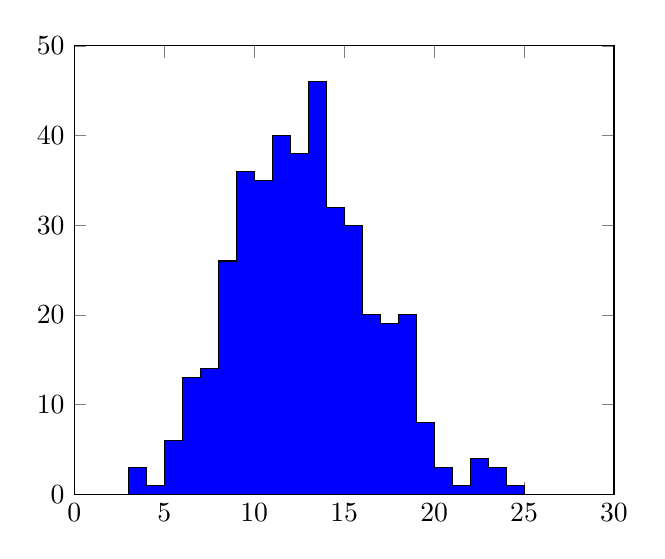
\begin{tikzpicture}
\begin{axis}[xmin = 0, xmax = 30,ymin=0, ymax=50,enlargelimits=false]
\addplot [
const plot,
fill=blue,
draw=black,
] coordinates {
(3, 3)
(4, 1)
(5, 6)
(6, 13)
(7, 14)
(8, 26)
(9, 36)
(10, 35)
(11, 40)
(12, 38)
(13, 46)
(14, 32)
(15, 30)
(16, 20)
(17, 19)
(18, 20)
(19, 8)
(20, 3)
(21, 1)
(22, 4)
(23, 3)
(24, 1)
(25, 1)

}
\closedcycle
;
\end{axis}
\end{tikzpicture}
\end{center}


\begin{center}
Гистограммы $W_n = f(n)$ для $\tau = 20$ и 40с.

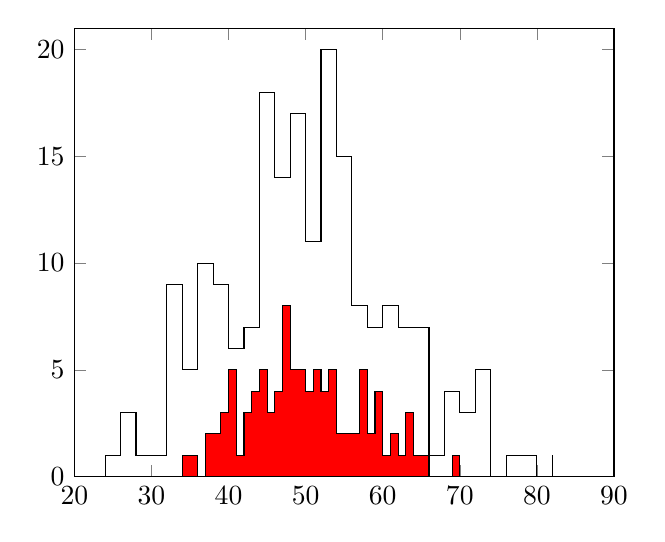
\begin{tikzpicture}
\begin{axis}[xmin = 20, xmax = 90,ymin=0, ymax=21,enlargelimits=false]
\addplot [
const plot,
fill=red,
draw=black,
] coordinates {
(34, 1)
(35, 1)
(36, 0)
(37, 2)
(38, 2)
(39, 3)
(40, 5)
(41, 1)
(42, 3)
(43, 4)
(44, 5)
(45, 3)
(46, 4)
(47, 8)
(48, 5)
(49, 5)
(50, 4)
(51, 5)
(52, 4)
(53, 5)
(54, 2)
(55, 2)
(56, 2)
(57, 5)
(58, 2)
(59, 4)
(60, 1)
(61, 2)
(62, 1)
(63, 3)
(64, 1)
(65, 1)
(66, 0)
(67, 0)
(68, 0)
(69, 1)
(70, 1)

}\closedcycle;

\addplot [
const plot,
draw=black,
] coordinates {
(12*2, 1)
(13*2, 3)
(14*2, 1)
(15*2, 1)
(16*2, 9)
(17*2, 5)
(18*2, 10)
(19*2, 9)
(20*2, 6)
(21*2, 7)
(22*2, 18)
(23*2, 14)
(24*2, 17)
(25*2, 11)
(26*2, 20)
(27*2, 15)
(28*2, 8)
(29*2, 7)
(30*2, 8)
(31*2, 7)
(32*2, 7)
(33*2, 1)
(34*2, 4)
(35*2, 3)
(36*2, 5)
(37*2, 0)
(38*2, 1)
(39*2, 1)
(40*2, 0)
(41*2, 1)

}\closedcycle;
\end{axis}
\end{tikzpicture}
\end{center}

Краткое пояснение по принципам расчета и постоения

Для совпадания центров необходимо увеличить значения количества частиц в $\frac{40s}{20s} = 2$ раза у данных для 20 с.

Данные для гистограмм с $\tau = 20$ и 40 с рассчитаю из соответствующих таблиц простым подсчетом числа тех или иных случаев.

Таблицу для $\tau = 40$ с получу попарным сложением элементов таблицы с $\tau = 20$ с.

11)Произведу расчеты. $\overline{n}$ рассчитаю для $\tau = 20$ с

\begin{equation}
\overline{n} = \sum^N_{i=1} n_i = 24.7
\end{equation}

Среднеквадратичная ошибка соответственно

\begin{equation}
\sigma_{\text{отд}} = \sqrt{\frac{1}{N} \sum^N_{i=1} \left( n_i - \overline{n} \right)^2} = 5.5
\end{equation}

12)Убедимся в справедливости формулы (5):

\begin{equation}
\sigma_{\text{отд}} = 5.5 \approx \sqrt{\overline{n}} = 5.0
\end{equation}

Значения близки в рамках одного порядка, а значит формула справедлива

13)Сделаю это для $\tau = 20$ с.

Из теории

\begin{equation}
\left\{
\begin{aligned}
\eta_{\sigma 1} = 68.3\%\\	
\eta_{\sigma 2} = 95.4\%
\end{aligned}
\right.
\end{equation}

На практике же(рассматривая случаи $24.7 \pm 5.0$ и $24.7 \pm 10.0$)

\begin{equation}
\left\{
\begin{aligned}
\eta_{r1} = \frac{131}{200}\cdot 100\% = 65.5\%\\	
\eta_{r2} = \frac{187}{200}\cdot 100\% = 93.5\%
\end{aligned}
\right.
\end{equation}

Расхождение наблюдается, но оно в рамках несовпадения 2-х ранее полученных значений ошибки.

16)Среднеквадрадратичные ошибки связаны с количеством зарегестрированных частиц за измерение по формуле

\begin{equation}
\sigma = \sqrt{n}
\end{equation}

Для сравнения надо использовать среднее значение n - $\overline{n}$.

Тогда ошибки измерений соотносятся как

\begin{equation}
\sigma_{10} : \sigma_{20} : \sigma_{40} = 1 : \sqrt{2} : 2
\end{equation}

Полуширина связана с ошибкой по формуле

\begin{equation}
FWMH \approx \sqrt{2\ln{2}} \cdot \sigma
\end{equation}

\begin{center}
\newpage
Итого

\begin{tabular}[t]{|c|c|c|}
\hline
сек & $\sigma$ & FWMH \\
\hline
10 & 3.5 & 4.2\\
20 & 5.0 & 5.9\\
40 & 7.1 & 8.3\\
\hline
\end{tabular}
\end{center}

17)Использую формулу для стандартной ошибки

\begin{equation}
\sigma_{\overline{n}} = \frac{\sigma_{\text{отд}}}{\sqrt{N}}
\end{equation}

\begin{center}
Составлю итоговую таблицу

\begin{tabular}[t]{|c|c|c|c|}
\hline
сек & $\sigma_{\overline{n}}$ & $E_{\overline{n}}$ & итог \\
\hline
10 & 0.18 & $1.42\%$ & $(12.35 \pm 0.18)$\\
20 & 0.35 & $1.42\%$ & $(24.7 \pm 0.4)$\\
40 & 0.71 & $1.42\%$ & $(49.4 \pm 0.7)$\\
\hline
\end{tabular}
\end{center}

18**)Построим график по 3-м точкам

\begin{center}
\begin{tikzpicture}
\begin{axis}[
	xlabel     = $\sigma$, % label x axis
    ylabel     = $\tau$ \text{, сек}, % label y axis
	xmin = 0, ymin = 0
	]
\addplot[mark = *] table {
	x     y
0.18	10
0.35	20
0.71	40
0		0
};
\end{axis}
\end{tikzpicture}
\end{center}

Как видно, это прямая, что очевидно из статистики


**Программа не выдавала данные, указанные в п8, поэтому я просто взял 3 полученные в процессе решения точки

\begin{bfseries}
	Вывод
\end{bfseries}

Считаю, что методы обработки статистических данных были успешно применены и цель работы выполнена


\end{problem}
\end{document}